\chapter{Continuous Function}

What does it mean for a function to be continuous?

Infinitely, this is some smoothness to the function i.g.,

\begin{center}
\begin{tikzpicture}
  \draw[->] (-1, 0) -- (4.2, 0) node[right] {$x$};
  \draw[->] (0, -1) -- (0, 4.2) node[above] {$f_1(x)$};
  \draw[scale=0.5, domain=-0.8:8, smooth, variable=\x] plot ({\x}, {\x});
\end{tikzpicture}

\begin{tikzpicture}
  \draw[->] (-1, 0) -- (4.2, 0) node[right] {$x$};
  \draw[->] (0, -1) -- (0, 4.2) node[above] {$f_2(x)$};
  \draw[-] (-0.5, 2) -- (0.5, 2);
  \draw[-] (0.5, 2) -- (1.5, 3);
  \draw[-] (1.5, 3) -- (2.5, 3);
  \draw[-] (2.5, 3) -- (3.5, 1.2);
  \draw[-] (3.5, 1.2) -- (4, 1);
\end{tikzpicture}
\end{center}

But, on the other hand 

\begin{center}
\begin{tikzpicture}
  \draw[->] (-1, 1) -- (4.2, 1) node[right] {$x$};
  \draw[->] (0, -1) -- (0, 4.2) node[above] {$f_3(x)$};
  \draw[-] (-0.5, 0) -- (1, 0);
  \draw[-] (1, 2) -- (4, 2);
  % \node[circle, draw] at (1, 0){};
  \node at (1, 0)[circle,fill,inner sep=1.5pt]{};
  \node at (1, 2)[draw,circle,fill=white,minimum size=4pt,inner sep=1.5pt]{};
\end{tikzpicture}
\end{center}

is not continuous

\section{Definition of Continuous Function}
\begin{definition}\label{def:contin}
    Let $f: \RR \lthen \RR$. We say $f$ is continuous at the point $x_0 \in \RR$ if there holds $\lim\limits_{x \to x_0}f(x) = f(x_0)$
\end{definition}

\begin{remark*}
    For $f$ to be continuous at $x_0 \in \RR$, we require
    \begin{enumerate}[(i)]
        \item $\lim\limits_{x \to 0} f(x)$ exists
        \item $\lim\limits_{x \to 0} f(x) = f(x_0)$
    \end{enumerate}
\end{remark*}

Another way of writing Definition~\ref{def:contin} is
\begin{definition*}[32]
    $f$ is continuous at $x_0$ if for all $\eps > 0$, $\exists\delta=\delta(\eps, x_0, f(x_0)) > 0$ such that
    $$|x-x_0| < \delta \implies |f(x) - f(x_0)| < \eps$$
\end{definition*}

\begin{example*}
    $f_3$ is not continuous at the point $x = 1$. 
\end{example*}
\begin{proof}
    Indeed, setting $\eps_0 = 1$, 
    we see that, given any $\delta > 0$, the point $x_\delta = 1 + \frac{\delta}{2}$ is such that $|x_\delta - 1| < \delta$ and $|f(x_\delta) - f(1)| = |1-(-1)|=2 > \eps_0$
\end{proof}

\begin{example*}
    $f(x) = x^2$ is continuous.
\end{example*}
\begin{proof}
    Indeed, let $x_0 \in \RR$ be any point and observe that
    \begin{align*}
        |f(x) - f(x_0)| &= |x^2-x_0^2| \\
        &= |(x+x_0)(x-x_0)| \\
        &= |x+x_0|\cdot|x-x_0|
    \end{align*}
    Let $\eps > 0$ be given. Now let $\delta = \min\left\{1, \frac{\eps}{2(1+|x_0|)}\right\}$, then
     \begin{align*}
        |x+x_0| &= |x-x_0+2x_0| \\
        &\leq |x-x_0| + 2|x_0| \\
        &\leq 1 + 2|x_0|
    \end{align*}
    Then provided $|x - x_0| < \delta$ we get
    $$|f(x) - f(x_0)| \leq (1 + 2|x_0|)\cdot\frac{\eps}{2(1 + |x_0|)} < \eps$$
\end{proof}
\begin{example*}
\[ f(x) =
  \begin{cases}
    0       & \quad  x = 0\\
    x \sin\left(\frac{1}{x}\right)  & \quad x \neq 0
  \end{cases}
\]
$f$ is continuous at $x = 0$
\end{example*}
\begin{proof}
    Indeed, let $\eps > 0$ be given and observe that 
    \begin{align*}
        |f(x) - f(0)| &= |x|\cdot\left|\sin\left(\frac{1}{x}\right)\right| \text{ for } x \neq 0 \\
        & \leq |x|
    \end{align*}
    So, letting $\delta(\eps) = \frac{\eps}{2}$, we see that
    $$|x-0| < \delta \implies |f(x)-f(0)| \leq \frac{\eps}{2} < \eps$$
\end{proof}

\section{Identity of Continuous Function}

\begin{lemma}
    Let $f, g: \RR \lthen \RR$ be continuous at $a \in \RR$. Then
    \begin{enumerate}[(i)]
        \item $f+g$ is continuous at $a$
        \item $f\cdot g$ is continuous at $a$
    \end{enumerate}
\end{lemma}
\begin{proof}
    We will prove each separately
    \begin{enumerate}[(i)]
        \item let $\eps > 0$ be given. By the definition of continuous, $\exists \delta_f = \delta_f(\eps, a) > 0$ such that 
        $$|x-a| < \delta_f \implies |f(x) - f(a)| < \frac{\eps}{2}$$
        and, $\exists \delta_g = \delta_g(\eps, a) > 0$ such that 
        $$|x-a| < \delta_g \implies |g(x) - g(a)| < \frac{\eps}{2}$$
        So, letting $\delta = \min\{\delta_f, \delta_g\}$, suppose $|x-a| < \delta$, we see that 
        \begin{align*}
            |f(x) + g(x) - (f(a) + g(a))| &\leq |f(x) - f(a)| + |g(x) - g(a)| \\
            &= \frac{\eps}{2} + \frac{\eps}{2} \\
            &= \eps
        \end{align*}
        \item let $\eps$ be given. Note that
        $$|f(x)g(x)-f(a)g(a)| \leq |g(x)|\cdot|f(x)-f(a)| + |f(a)|\cdot|g(x)-g(a)|$$
        Since $g$ is continuous at $a$, $\exists \delta_g = \delta_g(\eps, a) > 0$ such that
        $$|x-a| < \delta_g \implies |g(x)-g(a)| < \min\left\{1, \frac{\eps}{2(1 + |f(a)|)}\right\}$$
        Then, provided $|x-a| < \delta_g$, we get 
        $$|g(x)| \leq \overbrace{|g(x)-g(a)|}^{<1} + |g(a)| < 1 + |g(a)|$$
        Also, since $f$ is continuous at $a$, $\exists \delta_f = \delta_f(\eps, a) > 0$ such that
        $$|x-a| < \delta_f \implies |f(x) - f(a)| < \frac{\eps}{2(1 + |g(a)|)}$$
        Then, letting $\delta = \min\{\delta_f, \delta_g\}$, we see that whenever $|x-a| < \delta$, we have form
        $$|f(x)g(x) - f(a)g(a)| < (1 + |g(a)|)\left(\frac{\eps}{2(1 + |g(a)|)}\right) + |f(a)|\cdot\frac{\eps}{2(1 + |f(a)|)} < \eps$$
    \end{enumerate}
\end{proof}

\begin{lemma}
    Let $g: \RR \lthen \RR$ be continuous at $a \in \RR$ and $f: \RR \lthen \RR$ be continuous at $g(a)$. 
    Then $f \circ g$ is continuous at $a$
\end{lemma}

\begin{proof}
    Let $\eps > 0$ be given. Since $f$ is continuous at $g(a)$, $\exists \delta_f = \delta_f(\eps, a) > 0$ such that 
    $$|y - g(a)| < \delta_f \implies |f(y) - f(g(a))| < \eps$$
    Meanwhile, $g$ is continuous at $a$, so $\exists \delta_g = \delta_g(\delta_f(\eps, a), a) > 0$ such that
    $$|x - a| < \delta_g \implies |g(x) - g(a)| < \delta_f$$
    So, letting $\delta = \delta_g$, we see that
    \begin{align*}
        |x-a| < \delta &\implies |g(x) - g(a)| < \delta_f \\
        &\implies |f(g(x)) - f(g(a))| < \eps
    \end{align*} 
\end{proof}

\begin{lemma}
    Let $f: \RR \lthen \RR$ be continuous at $a$, and suppose $f(a) > 0$. 
    Then $\exists \delta > 0$ such that $f(x) > 0\ \forall x \in \left[a - \delta, a + \delta\right]$
\end{lemma}

\begin{proof}
    Since $f$ is continuous at $a$, $\exists \delta_f = \delta_f(a, \overbrace{f(a)}^\eps) > 0$ such that
    $$|x-a| < \delta_f \implies |f(x) - f(a)| < \overbrace{\frac{1}{2}f(a)}^\eps$$
    It follows that, for $x \in (a - \delta_f, a + \delta_f)$, we have
    \begin{align*}
        f(x) &= (f(x) - f(a)) + f(a) \\
        &\geq f(a) - |f(x) - f(a)| \\
        &> f(a) - \frac{1}{2}f(a) \\
        &= \frac{1}{2}f(a) > 0
    \end{align*}
    In turn, letting $\delta = \frac{1}{2}\delta_f$, we see that $f(x) > 0\ \forall x \in \left[a - \delta, a + \delta\right]$
\end{proof}


\section{Definition of Left/Right Continuity}

$f$ continuous on $(a, b)$ if $f$ is continuous at $x$, for all $x \in (a, b)$.
What does it mean for $f$ to be continuous at on $\left[a, b\right]$?
Should there be a difference between ``continuous on $(a, b)$" and ``continuous on $\left[a, b\right]$".

To gather intution, let's look at $f(x) = \frac{1}{x}$ on $(0, 1)$ and $\left[0, 1\right]$.

\begin{center}
    \begin{tikzpicture}
      \draw[->] (-1, 0) -- (4.2, 0) node[right] {$x$};
      \draw[->] (0, -1) -- (0, 4.2) node[above] {$f(x)$};
      \draw[scale=1, domain=0.3:3.5, smooth, variable=\x] plot ({\x}, {1/\x});
    \end{tikzpicture}
\end{center}

It's clar that $f$ is continuous at every point $a \in (0, 1)$ but $\lim\limits_{x \to 0}f(x)$ is not defined.
So, it ought to not be continuous on $\left[0, 1\right]$
We make the following define

\begin{definition*}[32]
    Let $f: \RR \lthen \RR$ and $a < b$ be real numbers.
    \begin{enumerate}[(i)]
        \item We say f is continuous on $(a, b)$ if $f$ is continuous at $x$ for every $x \in (a, b)$
        \item We say $f$ is continuous on $\left[a, b\right]$ if $f$ is continuous on $(a, b)$ and 
        $\lim\limits_{x \to a^+}f(x) = f(a)$ and $\lim\limits_{x \to b^-}f(x) = f(b)$
    \end{enumerate}
    We write $\lim\limits_{x \to a^+} f(x)$ to mean ``The limit $f$ as $x$ tends to $a$ from above''
    also written $\lim\limits_{x \searrow a} f(x)$
    and $\lim\limits_{x \to b^-} f(x)$ to mean ``The limit $f$ as $x$ tends to $b$ from below''
    also written $\lim\limits_{x \nearrow a} f(x)$
\end{definition*}

\begin{definition*}[32]\label{def:lfcts}
    Let $f: \RR \lthen \RR$ and $a \in \RR$
    \begin{enumerate}[(i)]
        \item We write $\mu = \lim\limits_{x \searrow a} f(x)$ if for all $\eps > 0$, $\exists\delta > 0$ such that
        whenever $a < x < a + \delta$ we have $|\mu - f(x)| < \eps$
        \item We write $\nu = \lim\limits_{x \nearrow a} f(x)$ if for all $\eps > 0$, $\exists\delta > 0$ such that
        whenever $a  - \delta< x < a$ we have $|\nu - f(x)| < \eps$
    \end{enumerate}
\end{definition*}
\begin{example*}
    Considered this graph 
    \begin{center}
        \begin{tikzpicture}
            \draw[-] (-1, 0) -- (1, 0) node[right] {};
            \draw[-] (4, 0) -- (6, 0) node[left] {};
            \node at (1, 1)[circle,fill,inner sep=1.5pt]{};
            \node at (4, 2)[circle,fill,inner sep=1.5pt]{};
            \node at (1, 0)[draw,circle,fill=white,minimum size=4pt,inner sep=1.5pt]{};
            \node at (4, 0)[draw,circle,fill=white,minimum size=4pt,inner sep=1.5pt]{};
            \draw (1, 1) sin (2, 2) cos (2.5, 1.5) sin (3, 1) cos (4, 2);
            \node[] at (1,-0.3) {$a$};
            \node[] at (4,-0.3) {$b$};
            \node[] at (0,1) {$f(a) = 1$};
            \node[] at (5,2) {$f(b) = 2$};
        \end{tikzpicture}
    \end{center}
    then, $\lim\limits_{x \searrow a} f(x) = 1$ and $\lim\limits_{x \nearrow b} f(x) = 2$
    on the other hand $\lim\limits_{x \nearrow a} f(x) = 0$ and $\lim\limits_{x \searrow b} f(x) = 0$
\end{example*}
\begin{example*}
    $\lim\limits_{x \to x_0} f(x)$ exists $\iff$ $\lim\limits_{x \nearrow x_0} f(x)$ and $\lim\limits_{x \searrow x_0} f(x)$ exists and are equal.
\end{example*}
    

\section{3 Hard Theorems}

\begin{theorem}[Intermediate Value Theorem]\label{thm:ivalt}
    Let $f: \RR \lthen \RR$ be continuous on $\left[a, b\right]$ for $a < b$.
    Suppose $f(a) < 0 < f(b)$
    Then $\exists \xi \in (a, b)$ such that $f(\xi)=0$
\end{theorem}

\begin{theorem}\label{thm:upbndcts}
    Let $f: \RR \lthen \RR$ be continuous on $\left[a, b\right]$ for $a < b$.
    Then $f$ is bounded above on $\left[a, b\right]$, i.e., $\exists M \in \RR$ such that $f(x) \leq M\ x \in \left[a, b\right]$
\end{theorem}

\begin{theorem}\label{thm:supbndcts}
    Let $f: \RR \lthen \RR$ be continuous on $\left[a, b\right]$.
    Then $\exists \xi \in \left[a, b\right]$ such that $f(x) \leq f(\xi)\ \forall x \in \left[a, b\right]$
    i.e., $f(\xi)=\sup\{f(x): x\in\left[a, b\right]\}$
    (we say that $f$ achieves its supremum on $\left[a, b\right]$)
\end{theorem}

\begin{lemma*}[$35'$]
    Let $f: \RR \lthen \RR$ and $b \in \RR$.
    Suppose $\lim\limits_{x \nearrow b} f(x) = f(b) > 0$
    Then $\exists \delta > 0$ such that $f(x) > 0$ for all $x \in (b - \delta, b)$
\end{lemma*}

\begin{proof}
    Directly from Definition 32(ii) (definition of $\lim\limits_{x \nearrow b} f(x)$) such that
    $$x \in (b - \delta, b) \implies |f(x) - f(b)| < \frac{1}{2} f(b)$$
    Then for such $x \in (b - \delta, b)$ we have 
    \begin{align*}
        f(x) &= (f(x) - f(b)) + f(b) \\
        & \geq f(b) - \overbrace{|f(x) - f(b)|}^{<\frac{1}{2}f(b)} \\
        &> \frac{1}{2} f(b) > 0
    \end{align*}
    Hence, for $x \in \left(b - \frac{\delta}{2}, b\right)$ we have $f(x) > 0$
\end{proof}

\begin{lemma*}[$35''$]
    Let $f: \RR \lthen \RR$ and $b \in \RR$.
    Suppose $\lim\limits_{x \searrow a} f(x) = f(a) > 0$
    Then $\exists \delta > 0$ such that $f(x) > 0$ for all $x \in (a, a + \delta)$
\end{lemma*}

\begin{proof}[Proof Theorem \ref{thm:ivalt}]
    Define the set $A=\{x \in \left[a, b\right]:f(y) < 0\ \forall y \in \left[a, x\right]\}$
    Since $f(a) < 0$, so $a \in A$, so $A \neq \emptyset$
    Also, using Lemma $35''$ $\exists \delta_1 > 0$ such that $f(y) < 0\ \forall y \in \left[a, a + \delta_1\right]$
    so $a + \delta_1 \in A$, and by Lemma $35'$ 
    $\exists \delta_2 > 0$ such that $f(y) > 0\ \forall y \in \left[b-\delta_2, b\right]$ where $b-\delta_2$ is an upper bound for $A$.
    So $A$ is bounded above and $\sup A$ is well-defined.
    Let $\alpha=\sup A$. We already know that $\alpha\in (a, b)$
    our aim is to show that $f(\alpha) \neq 0$
    We proceed by contradiction: 
    
    Suppose for contradiction that $f(\alpha) \neq 0$
    There are 2 possibilities
    \begin{enumerate}[(i)]
        \item $f(\alpha) < 0$
        \item $f(\alpha) > 0$
    \end{enumerate}
    Suppose (i) holds, Since $\alpha \in (a, b)$ and $f(\alpha) < 0$
    by \textbf{Lemma 35}, $\exists \delta_3 > 0$ such that $f(y) < 0\ \forall y \in \left[\alpha - \delta_3, \alpha + \delta_3\right]$
    But then $\alpha + \delta_3 \in A$ and $\alpha + \delta_3 > \alpha$

    Suppose (ii) holds. Then since $\alpha \in (a, b)$, $f(\alpha) > 0$ and $f$ is continuous. By \textbf{Lemma 35}, $\exists \delta_4 > 0$ such that $f(x) > 0\ \forall x \in \left[\alpha - \delta_4, \alpha+\delta_4\right]$
    But then $\alpha = \sup A$ by \textbf{Lemma 28} $\exists x_0 \in A$ such that $\alpha - \frac{\delta_4}{2} < x_0$
    Thus $x_0 \in (\alpha-\frac{\delta_4}{2}, \alpha) \subseteq \left[\alpha - \delta_4, \alpha+\delta_4\right] \implies f(x_0) > 0$
    But $x_0 \in A$ so $(f_x) < 0$
\end{proof}

\begin{corollary}
    Let $f: \RR \lthen \RR$ be continuous on $\left[a, b\right]$ and let $c\in\RR$.
    Suppose $f(a) < c < f(b)$. Then $\exists\xi \in (a, b)$ such that $f(\xi)=c$
\end{corollary}
\begin{proof}
    Define $g(x) = f(x) - c$ and apply \textbf{Theorem}~\ref{thm:ivalt} to $g$
\end{proof}

\begin{example}
    Let $f(x) = x^4 + x - 3\ \forall x \in \RR$
    \textbf{Fact}: all polynomials are continuous $\forall x \in \RR$
    A nice application of the Intermidiate Value Theorem is to find roots of continuous functions
    We can see by plugging in that 
    $$ f(1) = 1 + (-1) - 3 = -3$$
    $$ f(2) = 16 + 2 - 3 = 15$$
    IVT $\implies \exists x_0 \in (1, 2)$ such that $f(x_0) = 0$
    This  at least lets us estimate where roots are
\end{example}

\begin{example}
    Let $f(x) = x^4 + x - 3 + \tan\left(\frac{x}{2}\right)$ (continuous on $(-\pi, \pi)$)
    $$f(-1) = -3 - \tan\left(\frac{1}{2}\right) < 0$$
    $$f(2) = 15 - \tan\left(\frac{1}{2}\right) > 0$$
    IVT $\implies \exists x_0 \in (-1, 2)$ such that $f(x_0) = 0$
\end{example}


What is it useful for?
If we look at the set $f(\left[a, b\right]) = \{f(x) : x \in \left[a, b\right]\}$
and Theorem~\ref{thm:upbndcts} tell us that set is bounded.
Since the set is bounded, it has a supremum.
You can think of this as ``local max'' of $f$ on the interval $\left[a, b\right]$

Before proving Theorem~\ref{thm:upbndcts}, let's look at one of its consequences.

\begin{corollary}
    Let $f: \RR \to \RR$ be continuous on $\left[a, b\right]$.
    Then $f$ is bounded below on $\left[a, b\right]$, i.e.,
    $\exists m \in \RR$ such that $m \leq f(x)\ \forall x \in \left[a, b\right]$
\end{corollary}
\begin{proof}
    Since $f$ is continuous, so is $(-f)$. Now apply Theorem~\ref{thm:upbndcts} to $-f$.
    $\exists M \in \RR$ such that $-f(x) \leq M\ \forall x \in \left[a, b\right]$
    the, $f(x) \leq -M\ \forall x \in \left[a, b\right]$
\end{proof}

\textbf{Takeaway}: If $f$ is continuous on $\left[a, b\right]$, then $f$ is bounded above + below on $\left[a, b\right]$

To prove Theorem~\ref{thm:upbndcts}, we'll need a few Lemmas.
\begin{lemma}
    Let $f: \RR \to \RR$ is continuous at $a \in \RR$, then $\exists \delta > 0$ such that
    $f$ is bounded above on the interval $\left[a-\delta, a + \delta\right]$
\end{lemma}
\begin{proof}
    Since $f$ is continuous at $a$, $\exists \delta = \delta(a, \overbrace{1}^\eps)$ such that 
    $|x-a| < \delta \implies |f(x) - f(a)| < 1$
    This for such $x$ we have 
    \begin{align*}
        f(x) &= f(x) - f(a) + f(a) \\
        &\leq |f(x) - f(a)| + |f(a)| \\
        &< 1 + |f(a)|
    \end{align*}
    For $x$ satisfying $|x-a| < \delta$, we have $f(x) < 1 + f(a)$.

    In particular, $f(x) < 1 + f(a)\ \forall x \in \left[a-\frac{\delta}{2}, a + \frac{\delta}{2}\right]$ 
\end{proof}

\begin{lemma*}($43'$)
    Let $f: \RR \to \RR$ be a function and $b \in \RR$.
    Suppose $\lim\limits_{x \nearrow b} f(x) = f(b)$. 
    Then $\exists \delta > 0$ such that $f$ is bounded above on $\left[b-\delta, b\right]$
\end{lemma*}

\begin{proof}
    By Definition $32''$, $\exists \delta = \delta(b, 1)$ such that
    $$0 < |x-b| < \delta \implies |f(x) - f(b)| < 1$$
    Therefore, for such $x$, 
    \begin{align*}
        f(x) &= f(x) - f(b) + f(b) \\
        &\leq |f(x) - f(b)| + |f(b)| \\
        &< 1 + |f(b)|
    \end{align*}
    $f(x) < f(b) + 1\ \forall x \in \left[b-\frac{\delta}{2}, b\right]$
\end{proof}

\begin{lemma*}($43''$)
    Let $f: \RR \to \RR$ be a function and $a \in \RR$.
    Suppose $\lim\limits_{x \searrow a} f(x) = f(a)$. 
    Then $\exists \delta > 0$ such that $f$ is bounded above on $\left[a, a+\delta\right]$
\end{lemma*}

\begin{proof}[Proof Theorem~\ref{thm:upbndcts}]
    As in the proof of Theorem~\ref{thm:ivalt}, consider the set
    $$A = \{ x \in \left[a, b\right] : f \text{ is bounded above on }\left[a, x\right]\}$$
    Since $a \in A$, we know $a \neq \emptyset$.
    Moreover, the point $b$ is an upper bound for $A$, so $\sup A = \alpha$ exists.

    Our objective is to show that $\alpha = b$.

    Suppose for contradiction that $\alpha < b$.
    (Note that we must have $a < \alpha$.
    We can't have $a > \alpha$ since $a \in A$. and $\sup A \geq a$.
    If $\alpha = a$, then $A = \{a\}$, but we know from Lemma $43''$ that
    $\exists \delta > 0$ such that $\left[a, a+\delta\right] \subseteq A$)

    By assumption $a < \alpha < b$ and so Lemma $43$ $\implies \exists\delta > 0$ such that
    $f$ isbounded on $\left[\alpha - \delta, \alpha + \delta\right]$.
    Let's say $f(x) \leq m_2$ on this interval $\left[\alpha - \delta, \alpha + \delta\right]$.

    By Lemma 28 (Alternate definition of supremum)
    $\exists x_0 \in A$ such that $\alpha - \delta < x_0 \leq \alpha$.
    $f$ is bounded above on $\left[a, x_0\right]$ (by the definition of $A$).
    say $f(x) \leq m_1$ on $\left[a, x_0\right]$
    \begin{center}
    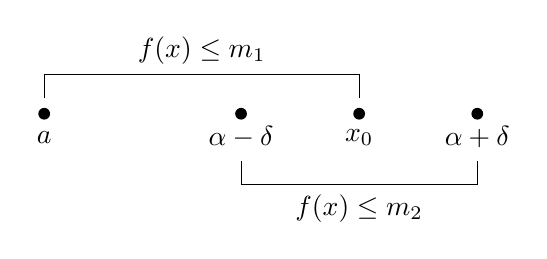
\begin{tikzpicture}
        \draw[-] (0, 0.5) -- (4, 0.5);
        \draw[-] (0, 0.5) -- (0, 0.2);
        \draw[-] (4, 0.5) -- (4, 0.2);
        \node at (2, 0.8) {$f(x) \leq m_1$};
        \node at (0, 0)[circle,fill,inner sep=1.5pt]{};
        \node at (0, -0.3){$a$};
        \node at (2.5, 0)[circle,fill,inner sep=1.5pt]{};
        \node at (2.5, -0.3){$\alpha - \delta$};
        \node at (4, 0)[circle,fill,inner sep=1.5pt]{};
        \node at (4, -0.3){$x_0$};
        \node at (5.5, 0)[circle,fill,inner sep=1.5pt]{};
        \node at (5.5, -0.3){$\alpha + \delta$};
        \draw[-] (2.5, -0.9) -- (5.5, -0.9);
        \draw[-] (2.5, -0.9) -- (2.5, -0.6);
        \draw[-] (5.5, -0.9) -- (5.5, -0.6);
        \node at (4, -1.2) {$f(x) \leq m_2$};
    \end{tikzpicture}
    \end{center}
    Thus, $f(x) \leq \max\{m_1, m_2\}\ \forall x \in \left[a, \alpha+\delta\right]$
    We deduce that $\alpha + \delta \in A$ and $\alpha + \delta > \alpha = \sup A$.
    Hence, 
    \begin{align*}
        \alpha = b &\iff \sup A = b \\
        &\implies f \text{ is bounded above on }\left[a, b\right] \text{ for every } x < b \text{ \circled{1}}
    \end{align*}
    Finally, using continuity at the point $b$ by Lemma $43'$ $\exists \delta'$ such that
    $f$ is bounded on $\left[b-\delta', b\right]$ \circled{2}.

    Hence, choosing $x = b - \delta'$ in \circled{1}, $\exists M$ such that $f(x) \leq M,\ \forall x \in \left[a, b - \delta'\right]$.
    and by \circled{2}, $\exists M_2$ such that $f(x) \leq M_2,\ \forall x \in \left[b-\delta', b\right]$.
    So, $f(x) \leq \max\{M, M_2\}\ \forall x \in \left[a, b\right]$.
\end{proof}

Summarize steps:
\begin{enumerate}[(i)]
    \item define a good set $A$
    \item show $b = \sup A$
    \item show $b \in A$
\end{enumerate}

The picture is 
\begin{center}
    \begin{tikzpicture}
        \draw[->] (-1, 0) -- (4.2, 0) node[right] {$x$};
        \draw[->] (0, -1) -- (0, 4.2) node[above] {$f(x)$};
        \draw[dotted] (-0.5, 3.2) -- (3.5, 3.2);
        \draw[-] (0.5, -0.1) -- (0.5, 0.1);
        \draw[-] (3.5, -0.1) -- (3.5, 0.1);
        \node at (0.5, -0.3){$a$};
        \node at (3.5, -0.3){$b$};
        \node at (-0.8, 3.2){$M$};
        \draw[dotted] (-0.5, -0.6) -- (3.5, -0.6);
        \node at (-0.8, -0.6){$m$};
        \draw (0.5, 1) sin (1.5, 3) cos (2, 1.25) sin (2.5, -0.5) cos (3.5, 2);
    \end{tikzpicture}
\end{center}

Whenever $f$ is continuous on $\left[a, b\right], \exists M > m$ such that 
$m \leq f(x) \leq M\ \forall x \in \left[a, b\right]$

\textbf{Note:} We must be careful aboue being continuous on $\left[a, b\right]$,
and mot just $(a, b)$. Indeed, $\substack{f:(0, 1)\lthen (0, \infty)\\
x\mapsto \frac{1}{x}}$, $f$ is continuous on $\left[\tilde{x}, \infty\right)$ for every $\tilde{x} > 0$,
but it is \underline{not} continuous on $\left[0, \infty\right)$.
    
\textbf{Question:} does these exists $\xi_1,\xi_2 \in \left[a, b\right]$ such that

$$f(\xi_1) = \inf_{\left[a, b\right]} f \text{ and } f(\xi_2) = \sup_{\left[a, b\right]} f$$

\textbf{Anwer:} Yes

Later on, when we discuss differentiability, if $\sup$/$\inf$ is achieved in $(a, b)$,
then $f' = 0$ at such points. This we will prove later. 

\begin{proof}[Proof of Theorm~\ref{thm:supbndcts}]
    We already know from Theorem~\ref{thm:upbndcts} that $f$ is bounded on $\left[a, b\right]$,
    i.e., the set $B = f(\left[a, b\right]) = \{f(x): x \in \left[a, b\right]\}$ is bounded.
    This set is nonempty and so $\beta = \sup B$ is well-defined;
    Since $\beta \geq f(x)\ \forall x \in \left[a, b\right]$ it suffies to show that
    $\exists \xi \in \left[a, b\right]$ such that $f(\xi) = \beta$.
    
    Suppose for contradiction that this is not the case, i.e., 
    $\beta \neq f(y)\ \forall y \in \left[a, b\right]$ Then the function $g: \left[a, b\right] \to \RR$,
    defined by $g(x) = \frac{1}{\beta - f(x)} \forall x \in \left[a, b\right]$,
    is well-defined and $g$ is continuous on $\left[a, b\right]$ by virtue of Lemma 33

    Since $g$ is continuous, by Theorem~\ref{thm:upbndcts}$\implies\ g$ is bounded above on $\left[a, b\right]$
    However, by Lemma 28, given any $n \in \NN, \exists x_n \in \left[a, b\right]$ such that 
    $$\beta - \frac{1}{n} < f(x_n)\leq \beta \implies g(x_n) \geq \frac{1}{\beta - \left(\beta-\frac{1}{n}\right)} = n$$ 

    Hence given any $n \in \NN, \exists x_n \in \left[a, b\right]$ such that $g(x_n) \geq n$ and
    therefore $g$ is unbounded on $\left[a, b\right]$.
\end{proof}

We've actually proved
\begin{corollary}\label{col:44}
    Let $f: \RR \to \RR$ be continuous on $\left[a, b\right]$. Then $\exists\xi \in \left[a, b\right]$ such that
    $f(\xi) = \sup\{f(x) : x \in \left[a, b\right]\}$ (we often write with the shorthand $\sup_{\left[a, b\right]} f$)
\end{corollary}

\begin{corollary}
    Let $f: \RR \to \RR$ be continuous on $\left[a, b\right]$. Then $\exists \xi \in \left[a, b\right]$ such that
    $f(\xi) = \inf\{f(x) : x \in \left[a, b\right]\}$ 
\end{corollary}

\begin{proof}
    Apploy Corollary~\ref{col:44} to the function $-f$ and use the result $\inf B = -\sup(-B)$.
\end{proof}

\begin{example}
    Suppose $f, g$ are continuous on $\left[a, b\right]$ and $f(a) < g(a)$ and $f(b) > g(b)$.
    Then $\exists x \in \left[a, b\right]$ such that $f(x) = g(x)$ (in actual fact, $x \in (a, b)$)
\end{example}

\begin{proof}
    define $h(x) = f(x) - g(x)$. Then $h$ is continuous on $\left[a, b\right]$,
    $h(a) < 0 < h(b)$ so from Theorem~\ref{thm:ivalt}, $\exists \xi \in (a, b)$ such that
    $h(\xi) = 0 \implies f(\xi)=g(\xi)$
\end{proof}

\begin{example}
    Suppose $f: \RR \to \RR$ is continuous on $\left[0, 1\right]$ and suppose 
    $0 \leq f(x) \leq 1\ \forall x \in \left[0, 1\right]$. Then $\exists x_0 \in \left[0, 1\right]$ 
    such that $f(x_0) = x_0$ (we can imagine that $f$ cross $y = x$)
\end{example}

\begin{proof}
    Note that if $f(0) = 0$ on if $f(1) = 1$, then we are done.
    Suppose that $f(0) \neq 0$ and $f(1) \neq 1$ then $0 < f(0)$ and $f(1) < 1$
    Let $g(x) = x - f(x)$. Then, $g(0) = 0 - f(0) < 0$ and $g(1) = 1 - f(1) > 0$.
    So, $g$ is continuous and $g(0) < 0 < g(1)$, where Theorem~\ref{thm:ivalt} 
    $\exists x_0 \in \left[0, 1\right]$ such that $g(x_0) = 0$ and hence $x_0 =f(x_0)$
\end{proof}
